\section{The Peg Solitaire Game}
\label{sec:peg-solitaire-game}

Peg solitaire represents a traditional puzzle typically played on either a cross-shaped board with 33 holes (commonly referred to as ``the English board") or a triangular board containing 15 holes.\cite{Bell_2006}

\subsection{Boards}
The game features multiple board layouts, each with its own unique characteristics and challenges:

\subsubsection{English Board}
The traditional English board is cross-shaped with 33 holes arranged in a distinctive pattern. The standard starting position has pegs in all holes except for the center, which is empty. The objective is to remove pegs by jumping over them until only one peg remains, ideally in the center position.

The English board layout is implemented in the code as follows:

\begin{center}
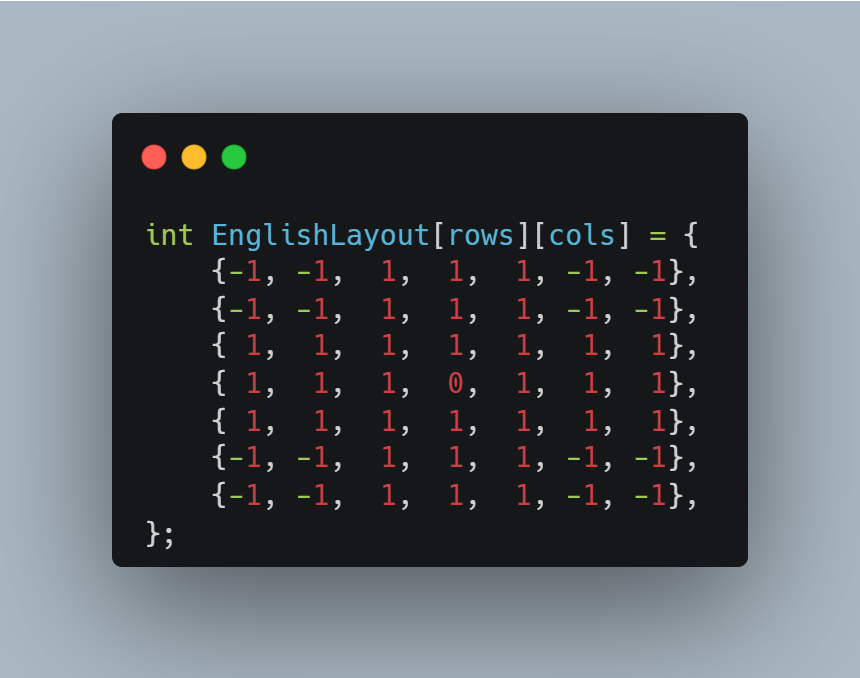
\includegraphics[width=0.5\textwidth]{resource/code-examples/EnglishLayout.png}
\end{center}

Where 1 represents a peg, 0 represents an empty hole, and -1 represents a position outside the board.

\subsubsection{Diamond Board}
The Diamond board is a compact, symmetrical layout with 41 holes arranged in a diamond pattern. The central hole is initially empty, and the goal remains the same as the English board—to finish with a single peg.

\subsubsection{Square Board}
The Square board provides a different challenge with a regular grid layout. This more geometrically uniform board offers different strategic considerations compared to the English and Diamond boards.

\subsubsection{Board Representation}
In the implementation, boards are represented using a two-dimensional grid structure,
and each cell in the grid can be in one of three states:

\begin{center}
    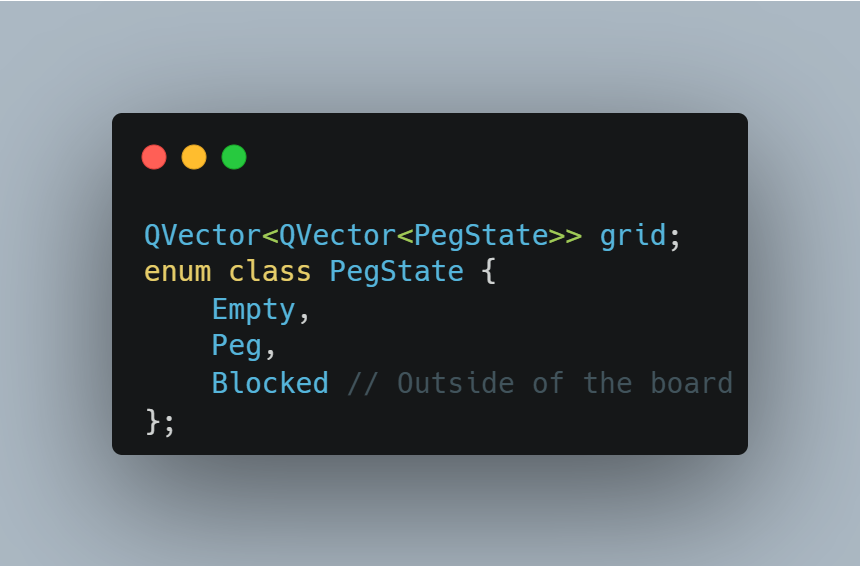
\includegraphics[width=0.5\textwidth]{resource/code-examples/BoardRepresentation.png}
\end{center}

\subsection{Special Game Rules}
In addition to the standard Peg Solitaire rules, the game includes special variants that provide novel gameplay experiences:

\subsubsection{Standard Rules}
In the classic Peg Solitaire game:
\begin{itemize}
    \item A peg can jump over an adjacent peg into an empty hole.
    \item The peg that is jumped over is removed from the board.
    \item Jumps can only be made horizontally or vertically, not diagonally.
    \item The goal is to clear the board until only a single peg remains.
    \item A "perfect" win is achieved when the final peg is in the center position.
\end{itemize}

\subsubsection{Anti-Peg Mode}
This innovative mode reverses the traditional gameplay mechanics:
\begin{itemize}
    \item The game begins with only one peg in the center of the board.
    \item A peg jumps over an empty space and lands on another empty space.
    \item After the jump, a new peg is placed in the empty space that was jumped over.
    \item The objective is to fill the board with as many pegs as possible.
    \item The game ends when no more moves are possible.
    \item A perfect win is achieved when only the starting position remains empty.
\end{itemize}

The Anti-Peg mode required significant code adaptations in checking move validity, as shown in this excerpt:

\begin{center}
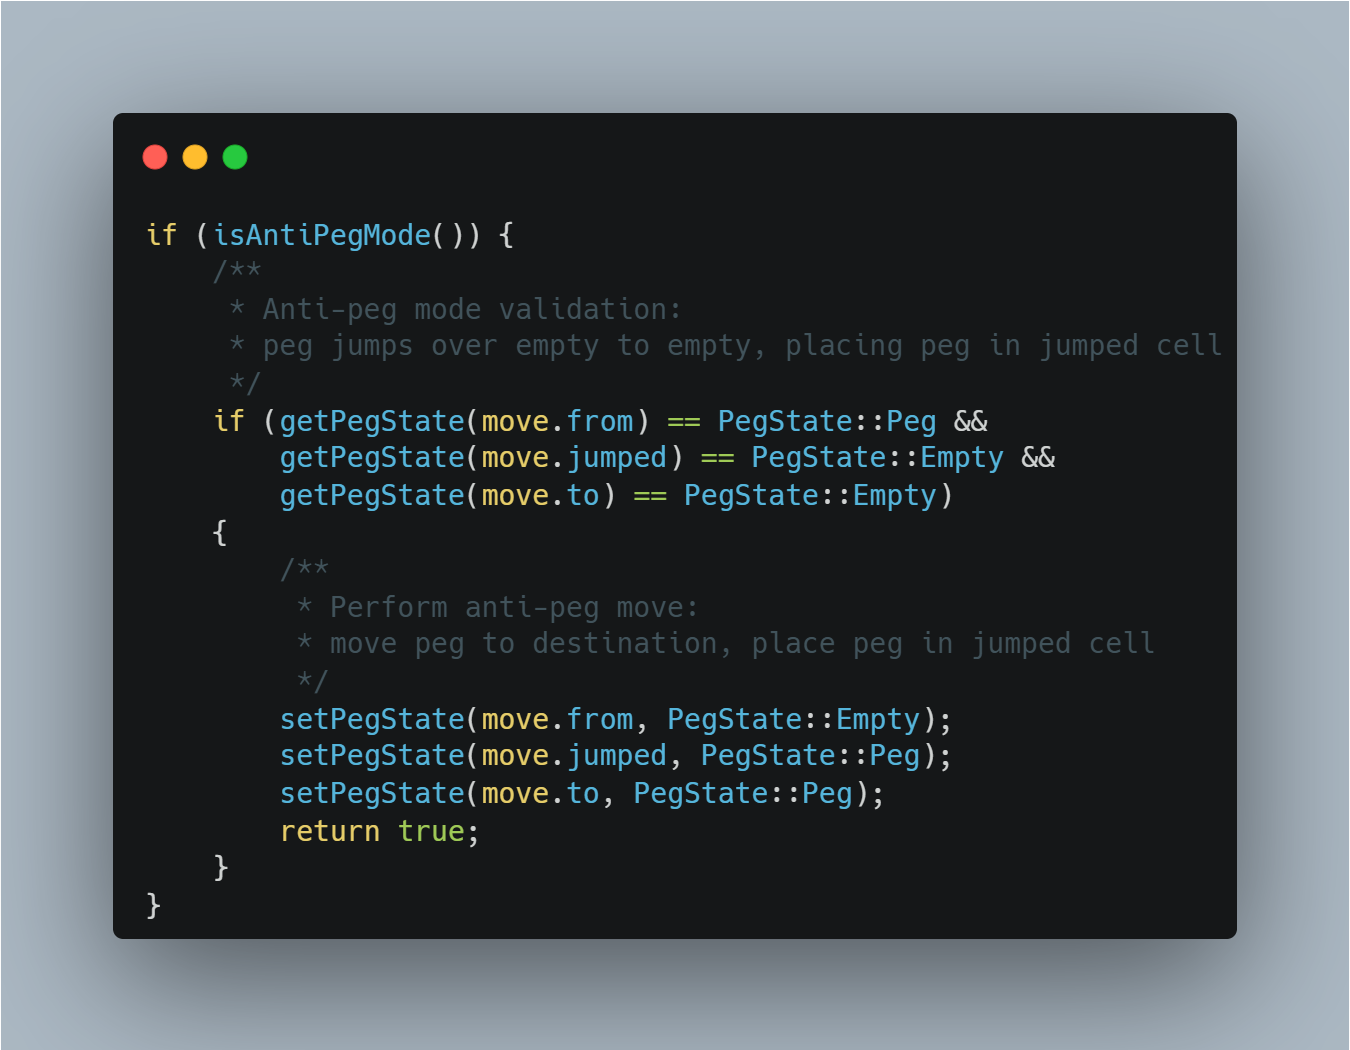
\includegraphics[width=0.6\textwidth]{resource/code-examples/AntiPeg.png}
\end{center}

\subsubsection{Endgame Mode}
The Endgame mode presents players with partially-completed board configurations:
\begin{itemize}
    \item The board is initialized with a random but solvable mid-game position.
    \item These positions are generated by working backward from a winning state.
    \item The algorithm applies 8-15 reverse moves from the winning position to create challenging puzzles.
    \item This guarantees that every puzzle has at least one solution.
    \item Players must analyze the position carefully to find the correct sequence of moves.
\end{itemize}

\subsection{Algorithm for Solving the Game}
Finding solutions to Peg Solitaire puzzles poses a significant computational challenge due to the vast number of possible move sequences. To address this, I implemented an optimized backtracking algorithm with several performance enhancements.\cite{Harder_PegSolitaire_2012}

\subsubsection{Depth-First Search with Backtracking}
The core solution algorithm uses depth-first search (DFS) with backtracking:
\begin{itemize}
    \item The algorithm recursively explores all possible move sequences from the current board state.
    \item At each step, it tries every valid move, makes the move, and then continues searching.
    \item If a dead end is reached, it backtracks and tries another move.
    \item The search terminates when a winning state is found (only one peg remains).
\end{itemize}

\subsubsection{Symmetry Optimization}

\begin{figure}[btp]
    \centering
    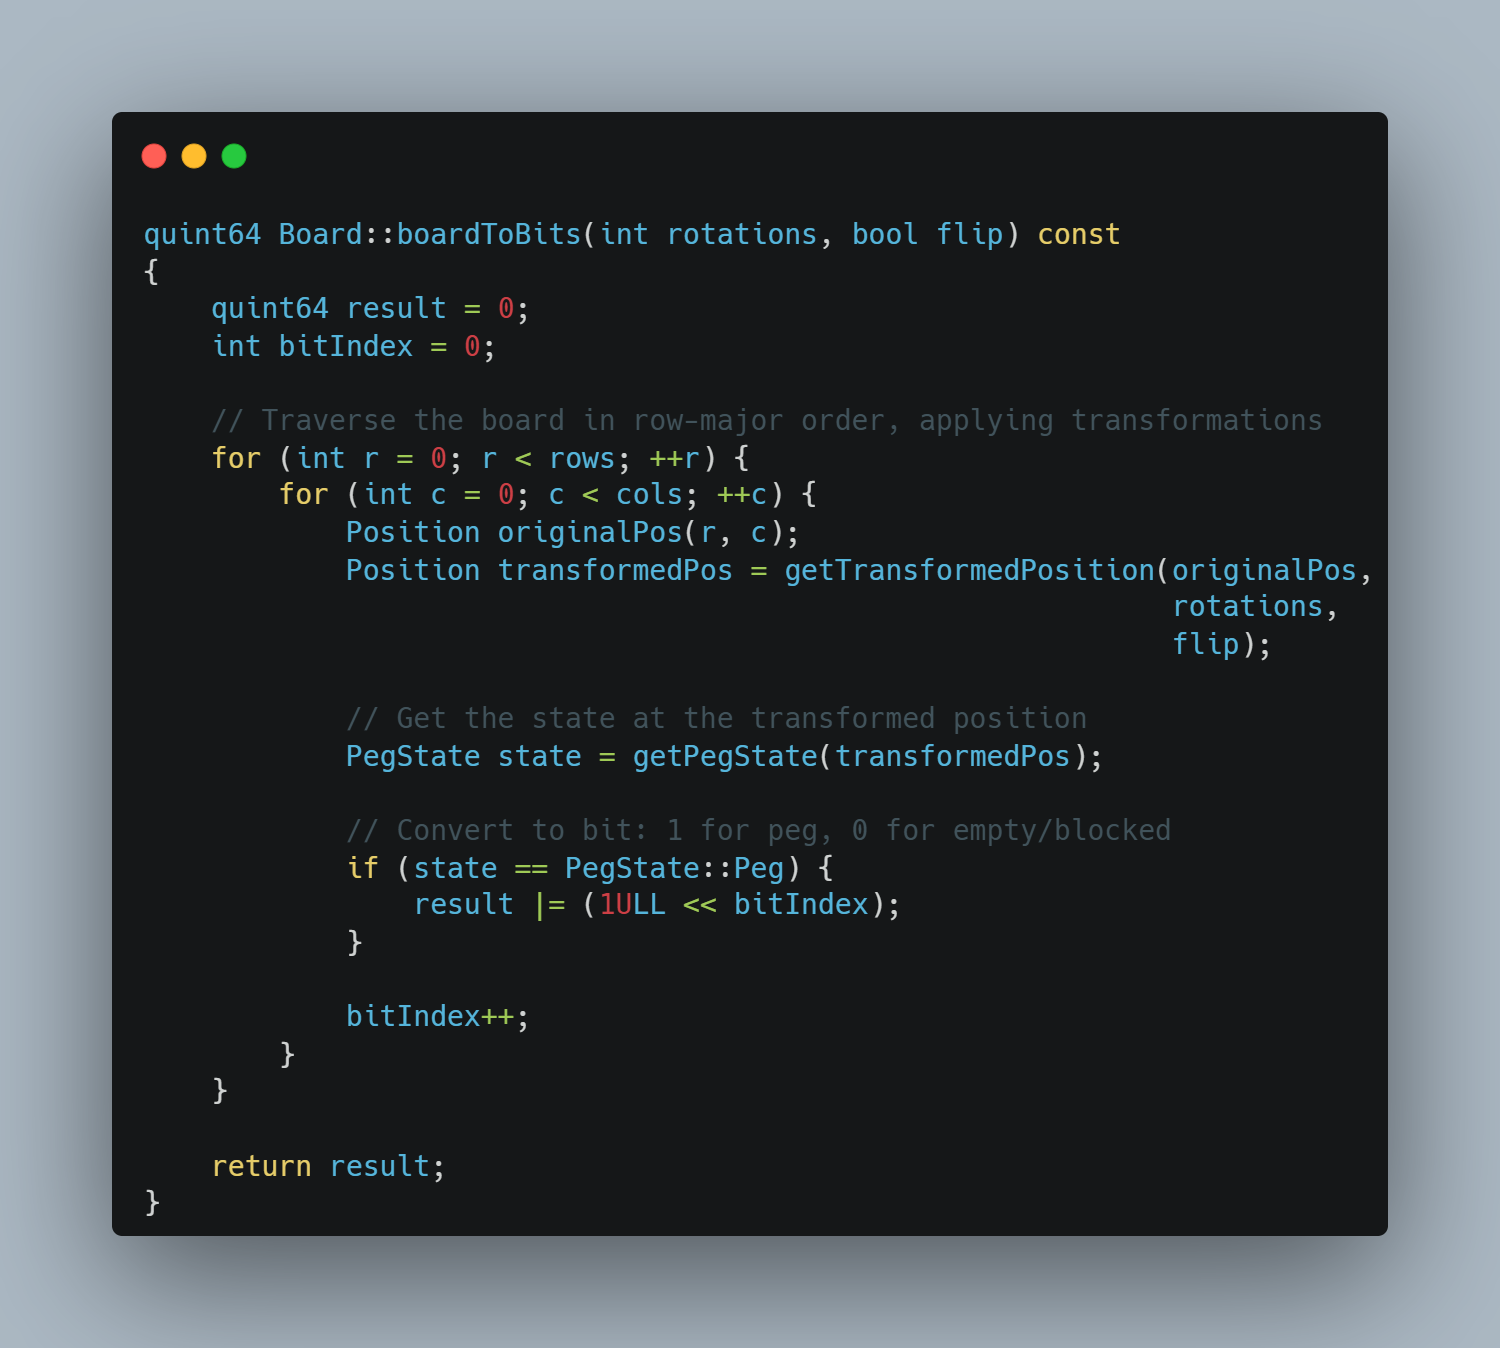
\includegraphics[width=0.45\textwidth]{resource/code-examples/boardToBits.png}
    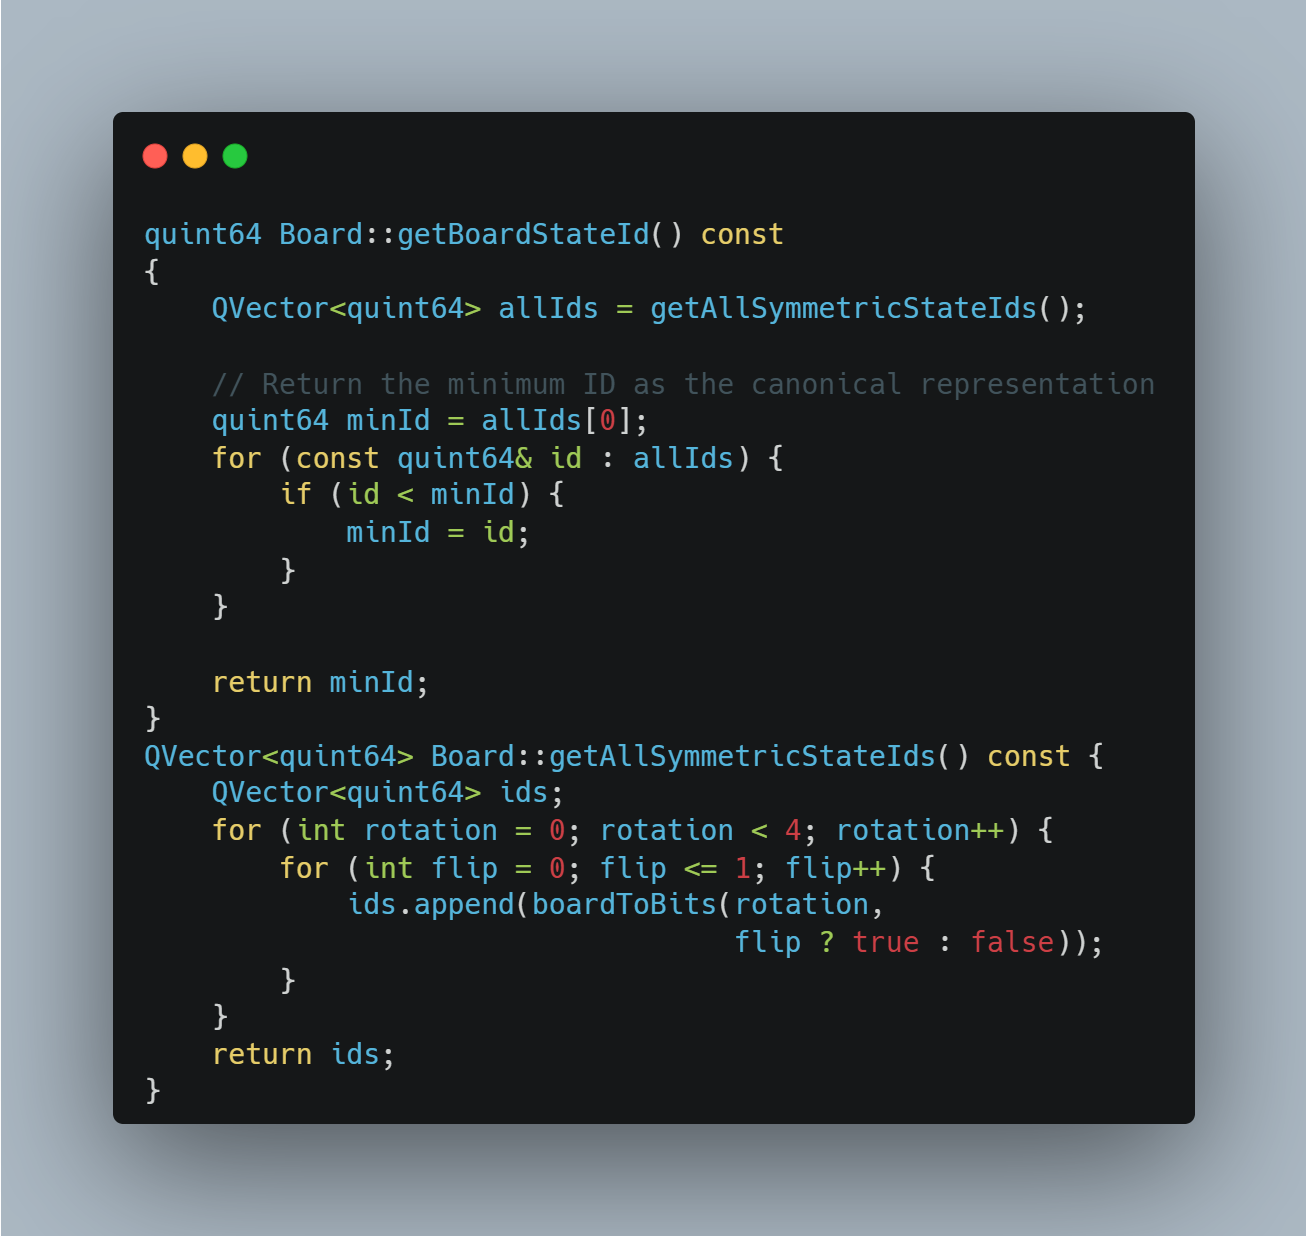
\includegraphics[width=0.45\textwidth]{resource/code-examples/getBoardStateId.png}
    \caption{Functions for computing board state identifiers.}
    \label{fig:board-state-id}
\end{figure}

A key innovation in the algorithm is the exploitation of board symmetry to drastically reduce the search space:
\begin{itemize}
    \item The English board has 8 symmetrical variants (4 rotations × 2 reflections).
    \item Many board states are equivalent under rotation and reflection.
    \item By identifying and storing these symmetric states, the algorithm avoids redundant exploration.
    \item A unique 64-bit identifier is computed for each board state and its symmetrical variants.
\end{itemize}

The board identifier is implemented using the functions shown in Figure \ref{fig:board-state-id}.

\subsubsection{Memoization}
To further enhance performance, the algorithm uses memoization to avoid recomputing results for previously seen states:
\begin{itemize}
    \item A static cache stores board states that have already been determined to be unsolvable.
    \item Before starting the search for a new position, the algorithm checks if the position (or any of its symmetric variants) is in the cache.
    \item This pruning technique significantly reduces the search space for complex positions.
\end{itemize}

\subsubsection{Multi-threaded Strategy Computation}
To maintain UI responsiveness while computing solutions, strategy calculations are offloaded to a separate worker thread:
\begin{itemize}
    \item A \texttt{StrategyWorker} class handles the computational workload asynchronously.
    \item The main UI thread remains responsive during intensive calculations.
    \item A loading animation provides visual feedback to the user during computation.
    \item The worker can be interrupted if the board state changes or the user requests a different action.
\end{itemize}

These algorithmic optimizations transform an intractable problem (which might take hours to solve with naive backtracking) into one that can be solved in a reasonable amount of time for most board states, making the strategy assistant feature practical for real-time use.